% --- SEZIONE 1: COMPONENTI DI SISTEMA E CONTROLLO ---

\section{Componenti del Sistema (SCS)}

\begin{itemize}
    \item \textbf{HardFaults:} Sempre attivati; gestiscono errori di Bus, Usage e Memory Management. Permettono una reazione rapida agli errori critici.
    \item \textbf{Wake-up Interrupt:} Consente la disattivazione gerarchica dei componenti
     per ridurre il consumo energetico (modalità Sleep/Stop).
    \item \textbf{Memory Protection Unit (MPU):} Genera eccezioni in caso di accessi non autorizzati alla memoria.
    \item \textbf{Debug Unit:} Fornisce fino a 4 breakpoint hardware per il debugging del codice.\\
        Core Debug Control, Breakpoint Unit (BP), Data Watchpoint Unit (DWT), ROM Table
    \item Un contatore a \textbf{24-bit} che fornisce una base dei tempi costante per il sistema operativo o i cicli di programma.
\end{itemize}

\section{Stack e Gestione Memoria}
\begin{itemize}
    \item \textbf{Direzione:} Cresce verso indirizzi di memoria inferiori.
    \item \textbf{Stack Pointer (SP):} Punta sempre al "top of stack". vietato leggere o scrivere al di sotto di SP.
    \item \textbf{Allineamento:} allocato in step di 8 byte.
    \item \textbf{Velocità:} due volte più rapido del RAM/ROM pointer, SP è già disponibile.
\end{itemize}

\section{Confronto Architetture ARM Cortex}
\begin{description}
    \item[Cortex-A (Application):] Calcolo generico ad alte prestazioni (Linux/Android).
    \item[Cortex-R (Real-Time):] Bassa latenza e alta affidabilità (automotive/medico).
    \item[Cortex-M (Microcontroller):] Ridotto consumo energetico, interrupt deterministici.
\end{description}

\renewcommand{\arraystretch}{1.5}
\resizebox{\columnwidth}{!}{
\begin{tabular}{|l|c|c|c|c|c|c|c|c|}
\hline
\textbf{Core} & \textbf{Thumb} & \textbf{Thumb-2} & \textbf{HW Mult.} & \textbf{HW Div.} & \textbf{Math Sat.} & \textbf{DSP} & \textbf{FPU} & \textbf{Arch} \\
\hline
Cortex-M0  & \cellcolor{green!60}Mostly & \cellcolor{green!60}Subset & \cellcolor{green!60}1/32 cyc & \cellcolor{red!60}No & \cellcolor{red!60}No & \cellcolor{red!60}No & \cellcolor{red!60}No & ARMv6-M \\
Cortex-M0+ & \cellcolor{green!60}Mostly & \cellcolor{green!60}Subset & \cellcolor{green!60}1/32 cyc & \cellcolor{red!60}No & \cellcolor{red!60}No & \cellcolor{red!60}No & \cellcolor{red!60}No & ARMv6-M \\
Cortex-M1  & \cellcolor{green!60}Mostly & \cellcolor{green!60}Subset & \cellcolor{green!60}3/33 cyc & \cellcolor{red!60}No & \cellcolor{red!60}No & \cellcolor{red!60}No & \cellcolor{red!60}No & ARMv6-M \\
Cortex-M3  & \cellcolor{green!60}Fully  & \cellcolor{green!60}Fully  & \cellcolor{green!60}1 cyc    & \cellcolor{green!60}Yes & \cellcolor{green!60}Yes & \cellcolor{red!60}No  & \cellcolor{red!60}No & ARMv7-M \\
Cortex-M4/M7  & \cellcolor{green!60}Fully  & \cellcolor{green!60}Fully  & \cellcolor{green!60}1 cyc    & \cellcolor{green!60}Yes & \cellcolor{green!60}Yes & \cellcolor{green!60}Yes & \cellcolor{yellow!60}Optional & ARMv7E-M \\
\hline
\end{tabular}}
\renewcommand{\arraystretch}{1}


\subsection{Evoluzione Cortex-M0 vs M0+}
\begin{minipage}[t]{0.49\columnwidth}
    \begin{itemize}
        \item \textbf{M0+ Pipeline:} Ridotta a 2 stadi per maggiore efficienza.
        \item \textbf{Accesso I/O:} Supporto per Single-Cycle GPIO.
        \item \textbf{Debugging:} Micro Trace Buffer (MTB) opzionale per il tracciamento dei salti.
        \item \textbf{MPU}
    \end{itemize}
\end{minipage}\hfill
\begin{minipage}[t]{0.49\columnwidth}
    \textbf{Pipeline}
    \begin{itemize}
        \item[+] Es wird in jedem Cycle ein Befehl ausgeführt
        \item [-] Bei sprüngen muss die Pipeline 'geleert' werden
    \end{itemize}
\end{minipage}

\section{Gestione degli Interrupt (NVIC)}

\begin{itemize}
    \item Il \textbf{Nested Vector Interrupt Controller} gestisce la prioritizzazione e il passaggio tra il programma di background e le \textbf{Interrupt Service Routine (ISR)}.
    \item \crd{L'LSB in ogni vettore indica la modalità di salto (1: thumb, 0: ARM) nei Cortex-M sempre 1} (Anche indirizzi in \texttt{LR} con \texttt{B..})
    \item Solitamente la VT (vector table) viene salvata in memoria fra il boot code e la seconda istruzione. 
    \item Tramite VTOR (Vector Table Offset Register) è possibile cambiare la posizione della tabella in memoria.
    \item \textbf{Stati dell'Interrupt:} \textit{Pending} (richiesto dalla periferica, azzerato automaticamente dall'hardware all'ingresso della ISR), \textit{Active} (in esecuzione in Handler Mode), \textit{Inactive}.
\end{itemize}

\subsection{NVIC Special Features}
\begin{itemize}
    \item \textbf{Tail-Chaining:} IRQ a bassa priorità è pendente al termine 
    di ISR attiva, la CPU salta l'Unstacking e lo Stacking. Fa solo un nuovo Vector Fetch 
    (da 15 $\rightarrow$ transizione di soli \textbf{6 cicli}).
    \item \textbf{Late Arrival:} IRQ ad alta priorità si attiva durante lo stacking 
    di un IRQ a bassa priorità, la CPU completa stacking ma esegue direttamente Vector Fetch dell'IRQ più urgente.
    \item \textbf{Pop-Preemption:} IRQ arriva durante l'Unstacking (Pop) finale, l'hardware abbandona il Pop e devia subito alla nuova ISR in soli \textbf{6 cicli}.
\end{itemize}\vspace{-1em}

\begin{minipage}[t]{0.5\columnwidth}
    \subsection{Registri di Mascheramento}
    \begin{itemize}
        \item \textbf{PRIMASK:} 1 bit. Disabilita tutti gli interrupt programmabili (tranne HardFault e NMI).
        \item \textbf{FAULTMASK:} 1 bit. Disabilita interrupt e tutte le eccezioni (tranne NMI).
        \item \textbf{BASEPRI:} Disabilita interrupt con priorità numerica maggiore o uguale (urgenza inferiore) a un valore impostato.
    \end{itemize}
    
    \subsection{Latenza e Stacking}
    \begin{itemize}
        \item \textbf{Interrupt Latency:} Tempo fisso d'ingresso nella ISR senza overhead software. \textbf{Cortex-M0+:} 15--16 cicli di clock. \textbf{Cortex-M3/M4:} 12 cicli.
        \item Le funzioni ISR sono di tipo \texttt{void ISR\_Handler(void)}: non accettano parametri e non restituiscono valori.
    \end{itemize}
    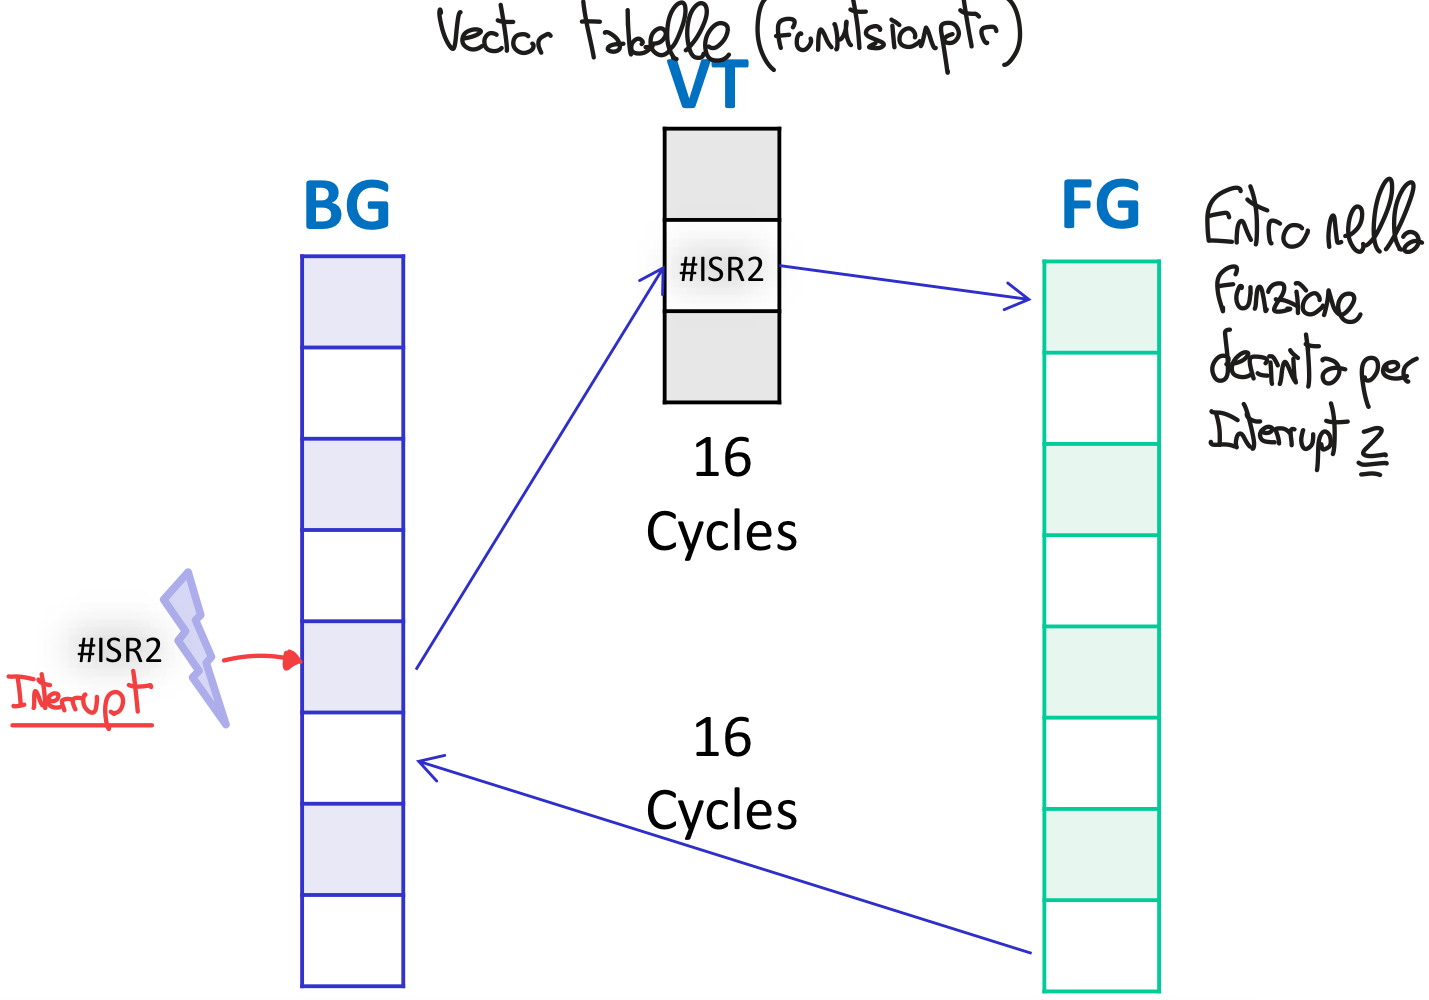
\includegraphics[width=\linewidth]{images/NVIC_sequence.png}
\end{minipage}
\hfill
\begin{minipage}[t]{0.49\columnwidth}
    \subsection{Preemption vs Subpriority}
    \begin{itemize}
        \item \textbf{Cortex-M0+:} Supporta solo 2 bit di priorità utilizzabili solo come Preemption.
        \item \textbf{Cortex-M3/M4:} Tramite il \textit{Priority Grouping}, gli 8 bit di priorità si dividono in:
        \begin{itemize}
            \item \textbf{Preemption bits:} Decidono se un interrupt può interrompere fisicamente una ISR in esecuzione (\textit{nesting}).
            \item \textbf{Subpriority bits:} Criterio di spareggio temporale se due IRQ arrivano insieme
        \end{itemize}
    \end{itemize}
    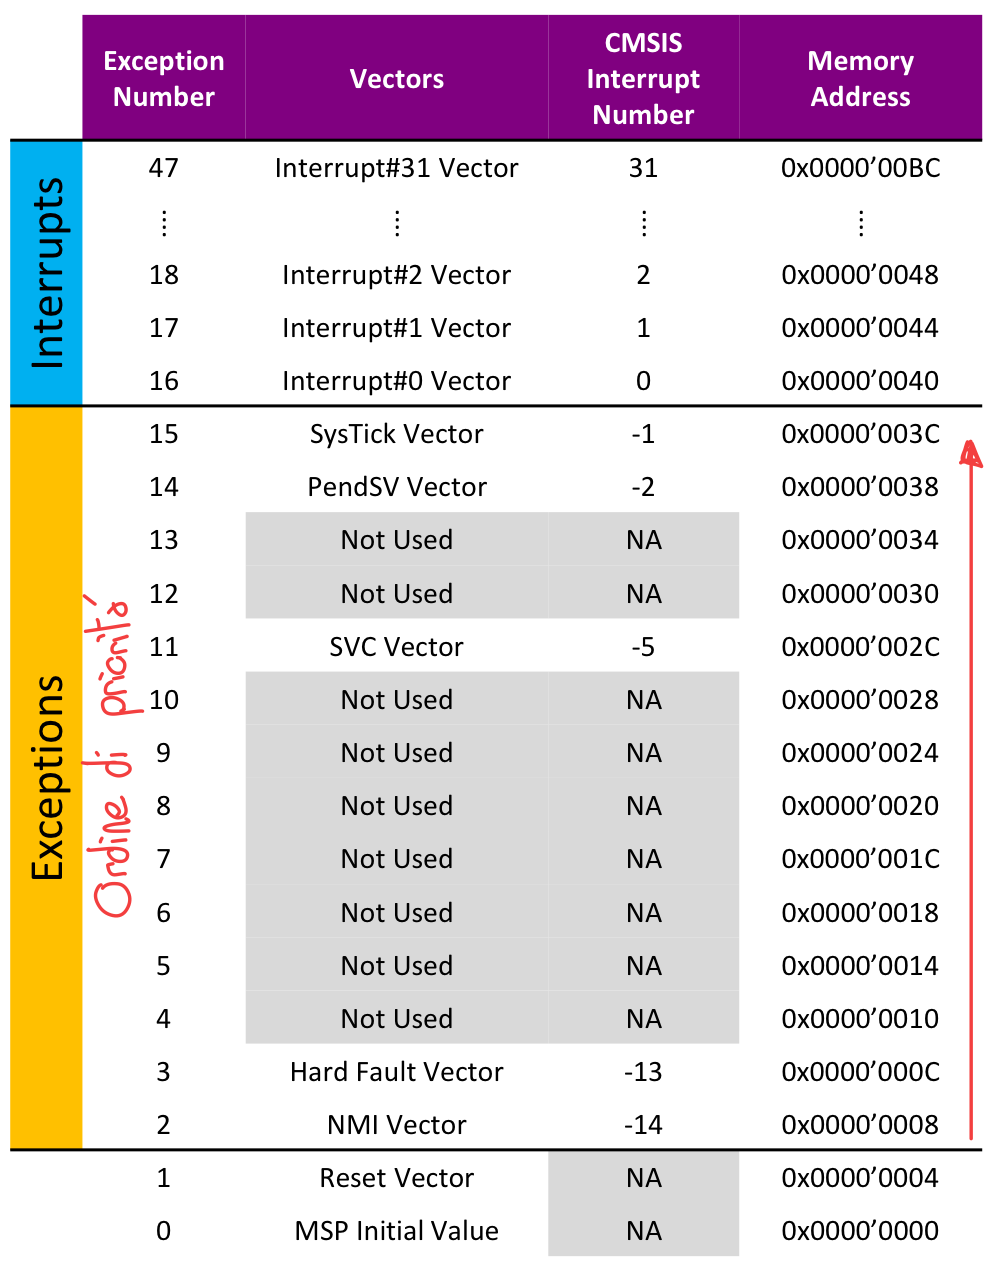
\includegraphics[width=0.98\linewidth]{images/NVIC_table.png}
\end{minipage}

\subsection{Soluzioni alternative \& Segnali IRQ}
\begin{minipage}{0.55\columnwidth}
    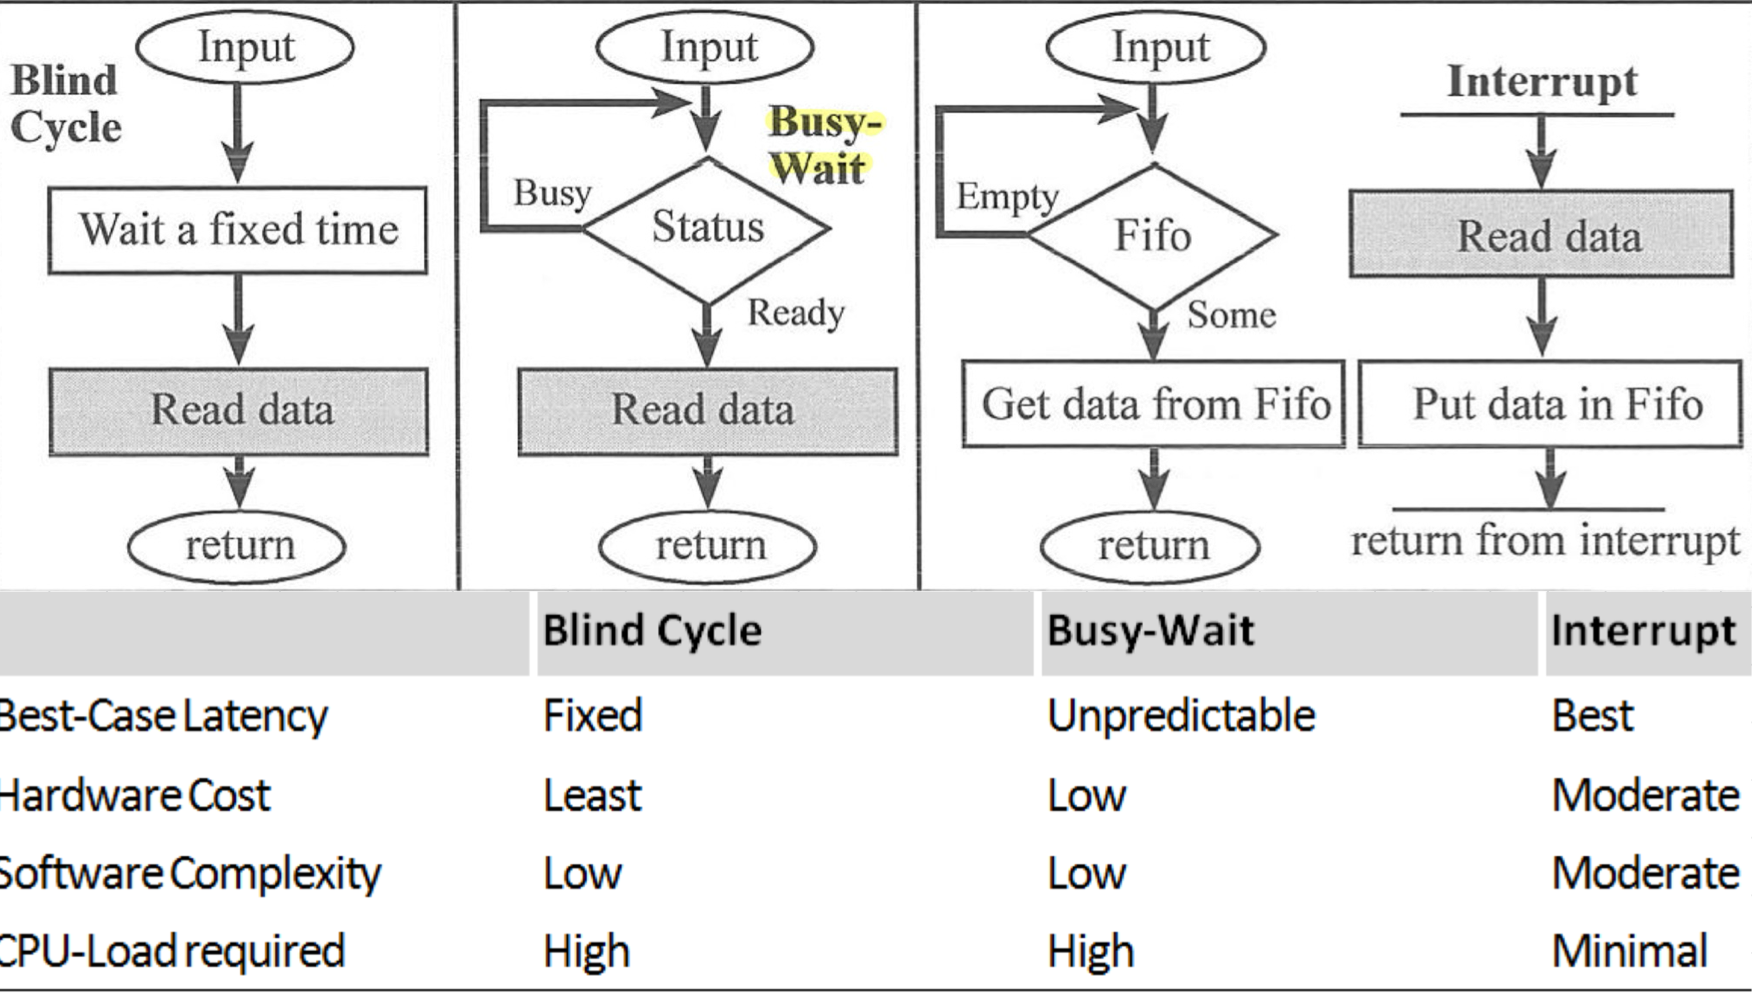
\includegraphics[width=\linewidth]{images/pooling_interrupts.png}
\end{minipage}
\begin{minipage}{0.45\columnwidth}
    \begin{enumerate}
        \item \textbf{Software Clearing}
        \item \textbf{Software Clearing mit Reset}
        \item \textbf{ISR Reentry (Pulsed IRQ durante ISR)}
        \item \textbf{Repulsed IRQ}
        \item \textbf{Pulsed IRQ (Level stay active)}
    \end{enumerate}
\end{minipage}

% Prima riga di immagini
\begin{minipage}[b]{0.49\linewidth}
    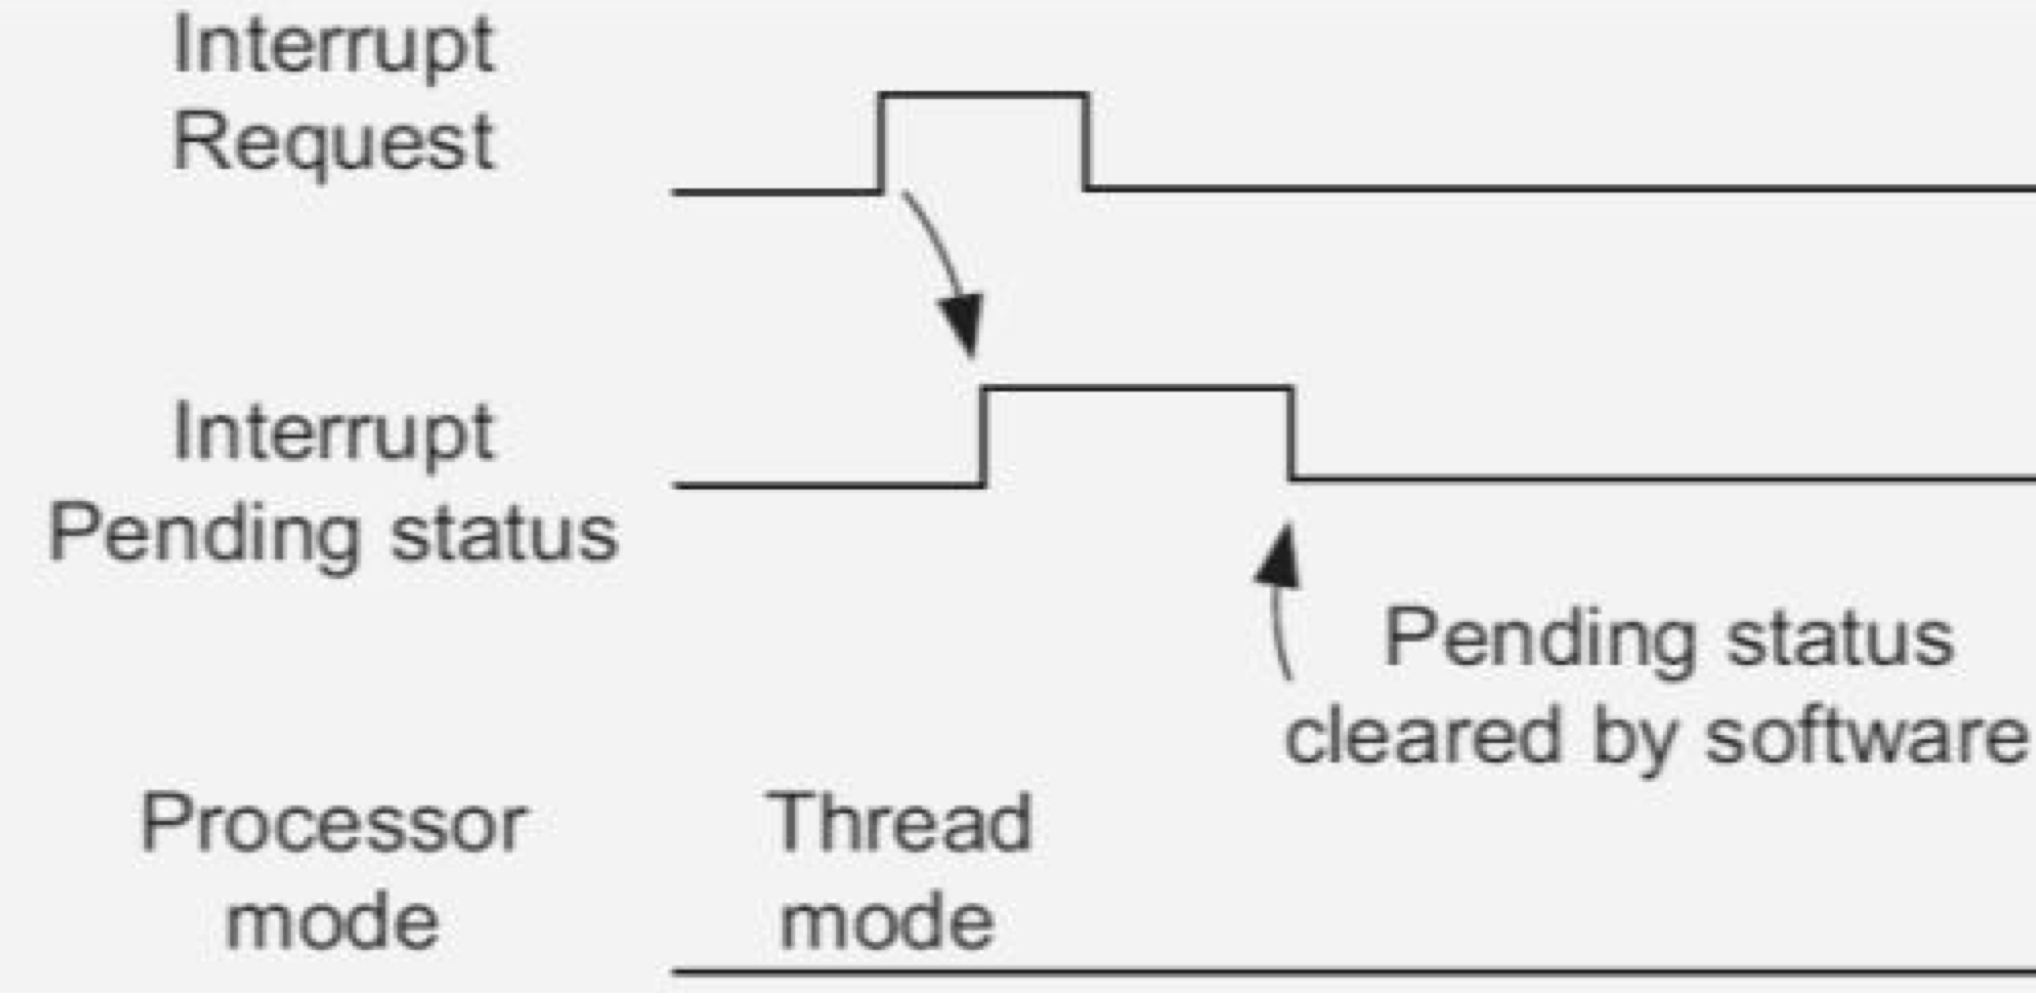
\includegraphics[width=0.8\linewidth]{images/software_clearing.png}
\end{minipage}
\begin{minipage}[b]{0.5\linewidth}
    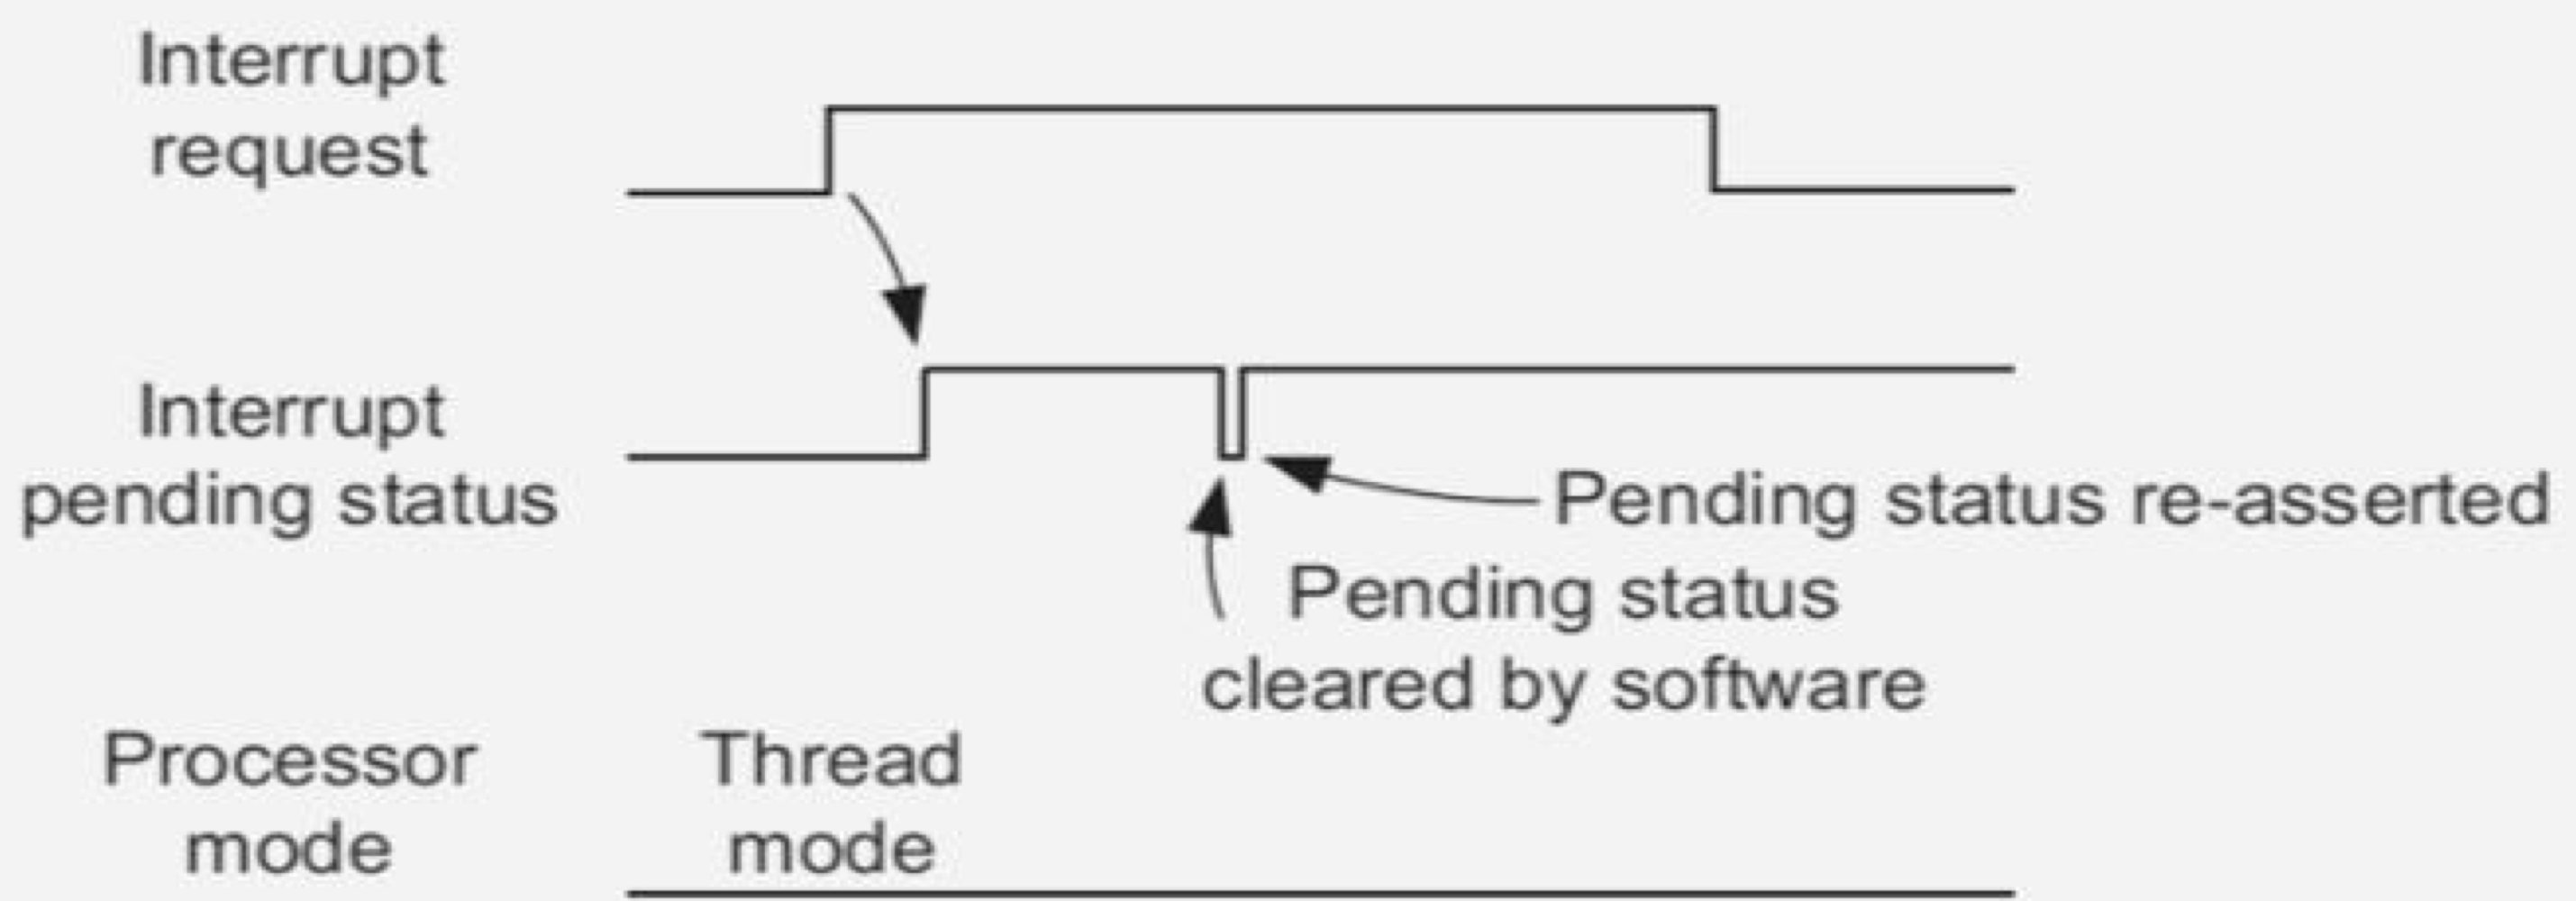
\includegraphics[width=\linewidth]{images/software_clearing_reset.png}
\end{minipage}

% Seconda riga di immagini
\begin{minipage}[b]{0.49\linewidth}
    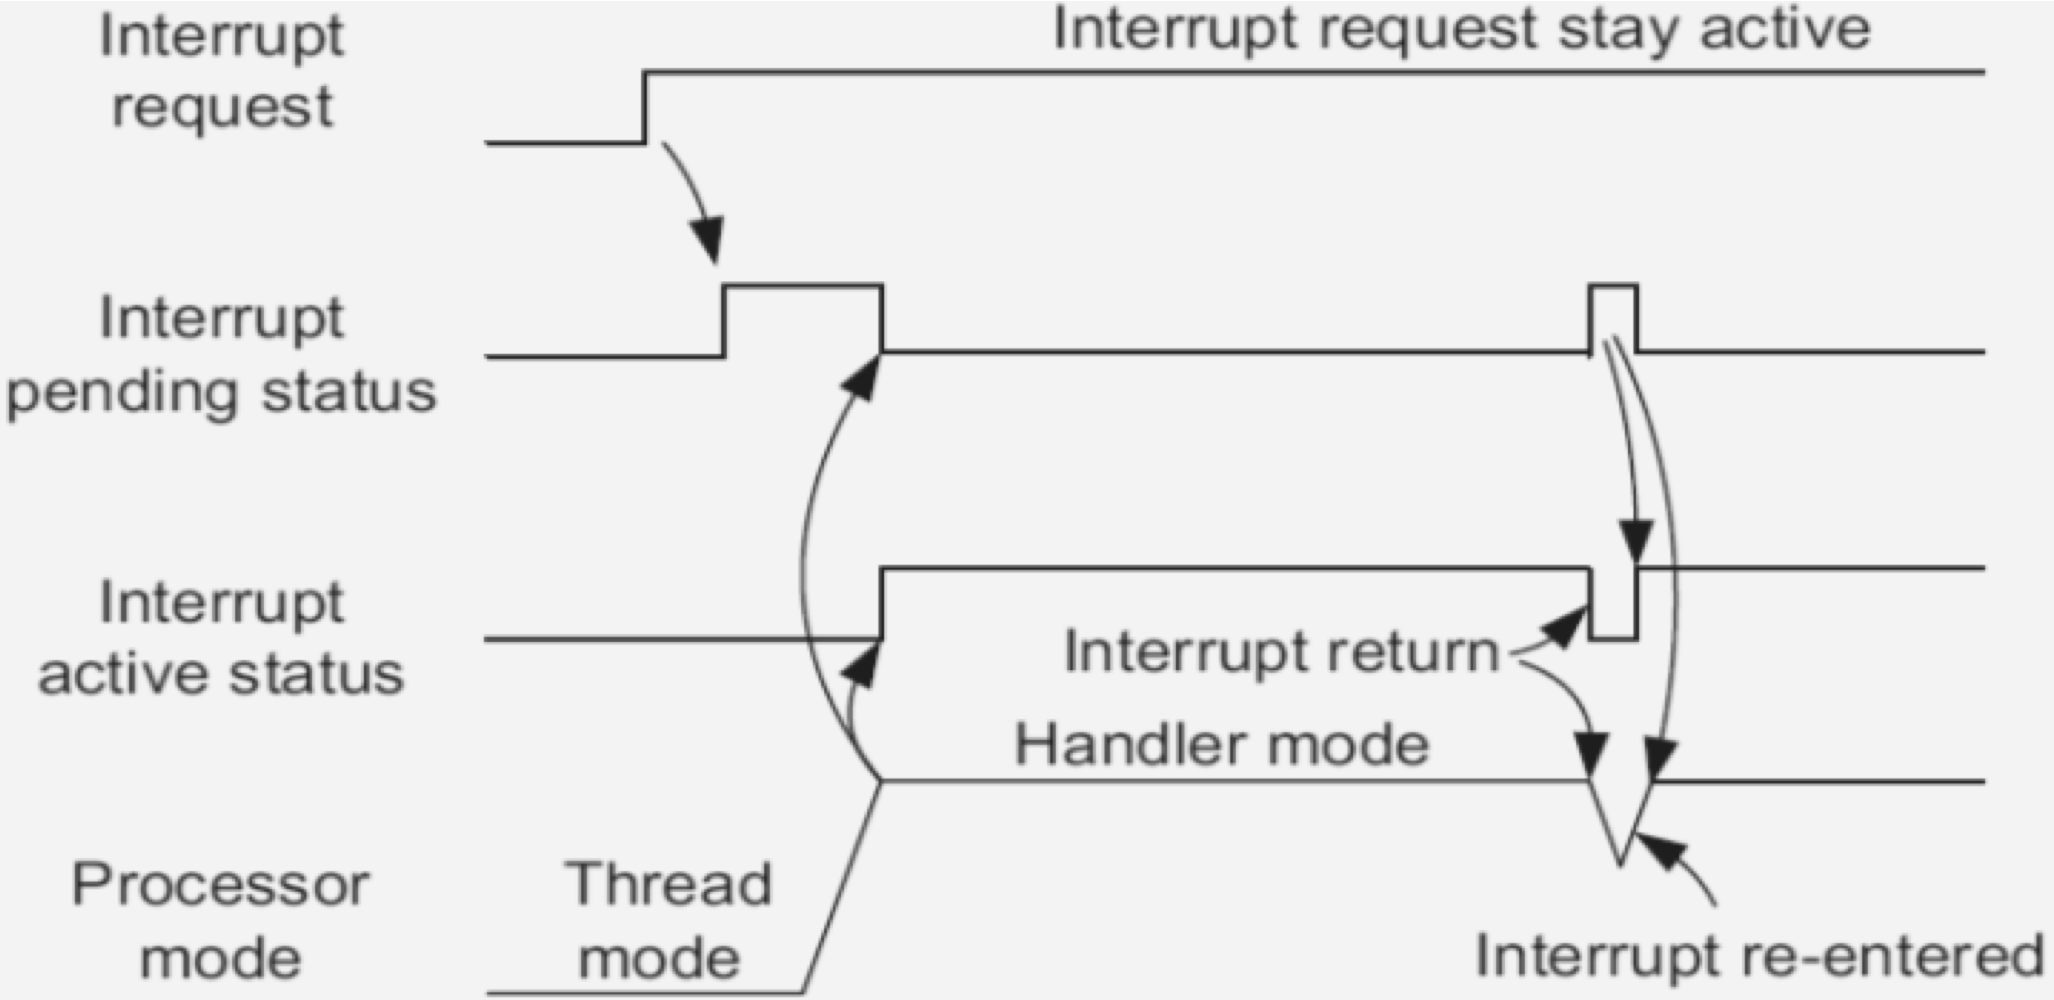
\includegraphics[width=\linewidth]{images/isr_reentry.png}
\end{minipage}
\begin{minipage}[b]{0.5\linewidth}
    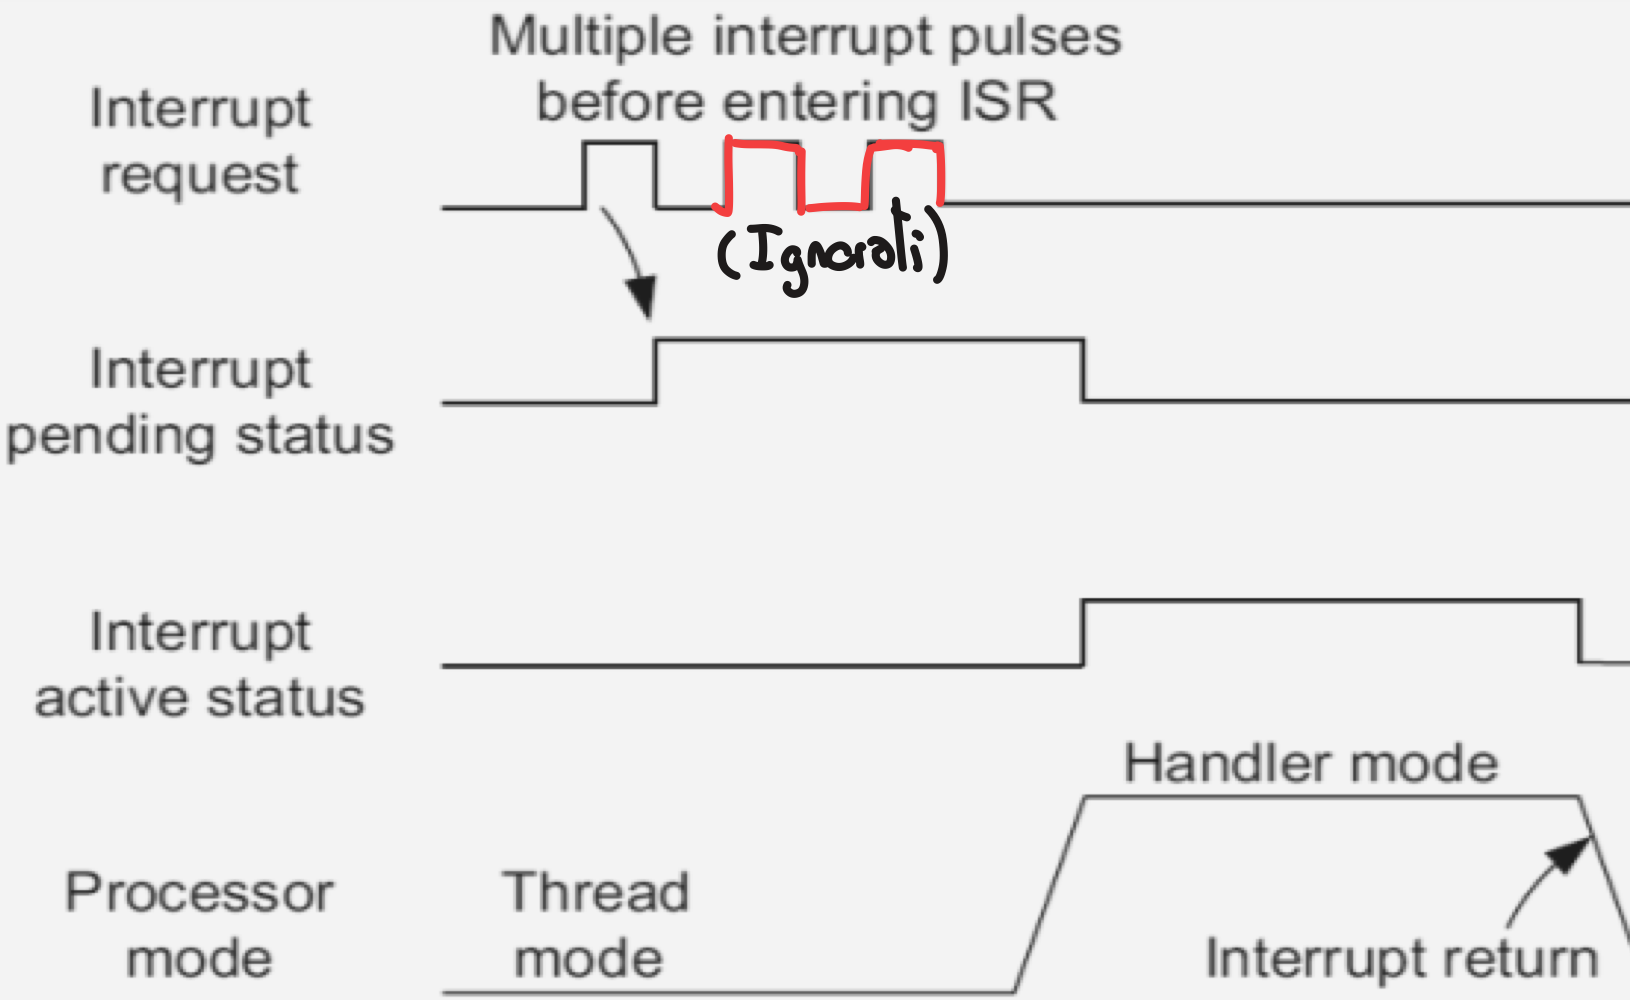
\includegraphics[width=0.9\linewidth]{images/repulsed_irq.png}
\end{minipage}

% Terza riga (ultima immagine centrata o a sinistra)
\begin{minipage}[t]{0.5\linewidth}
    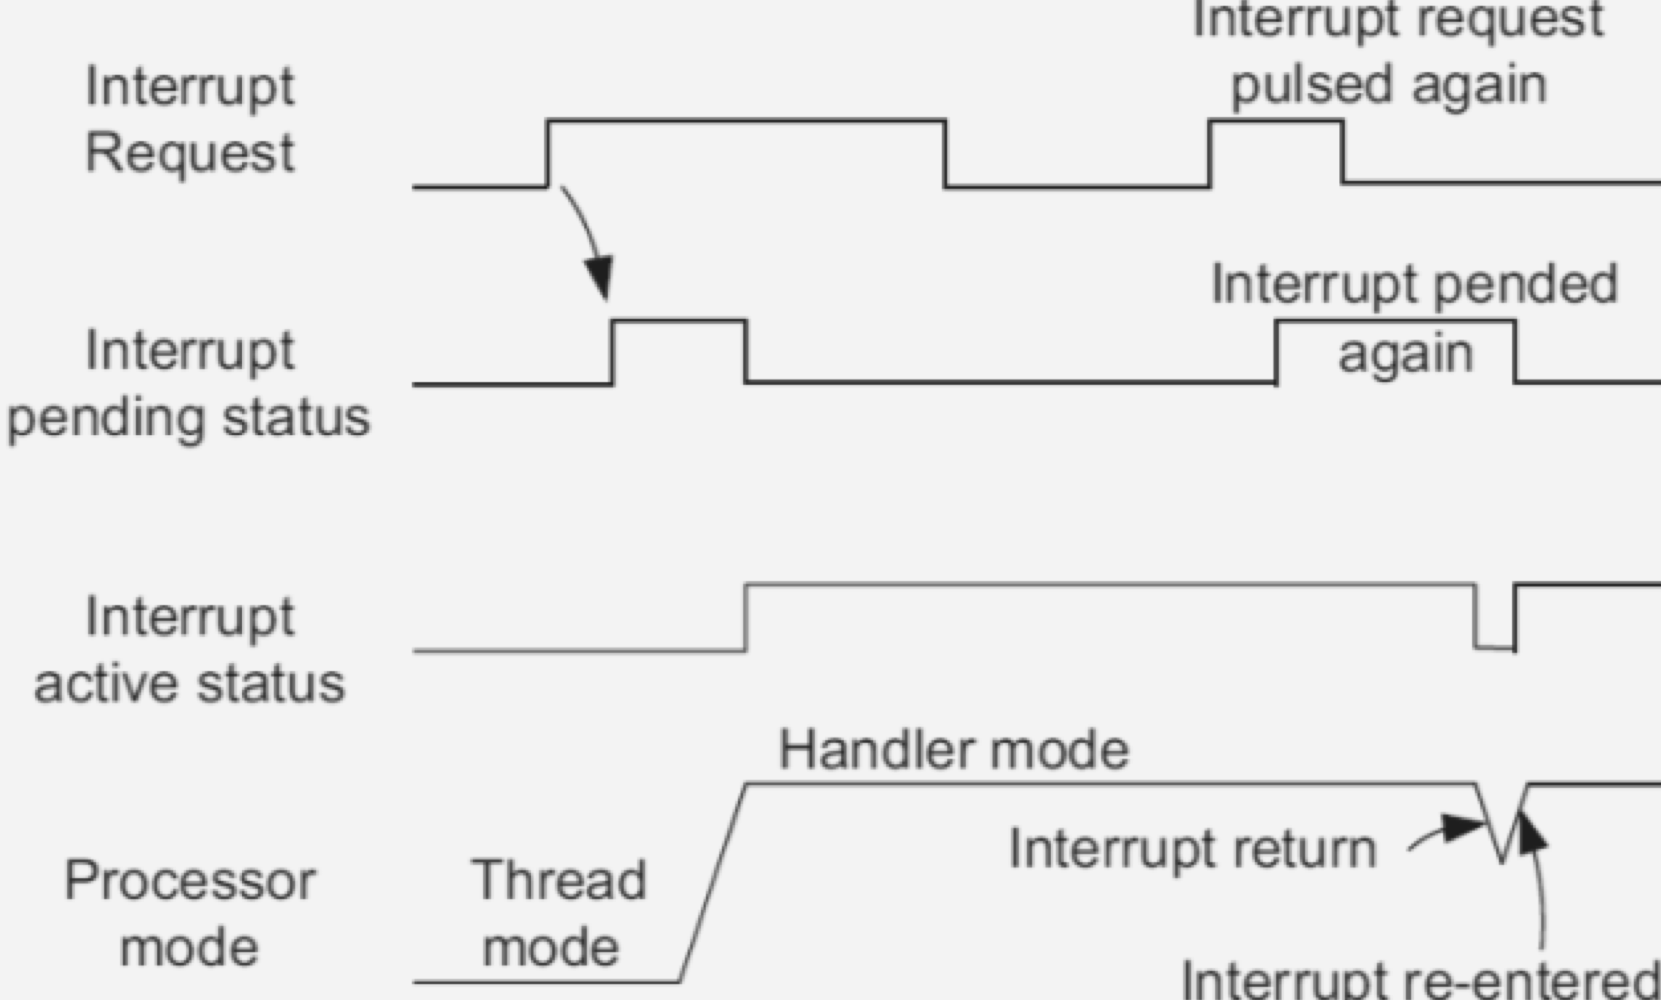
\includegraphics[width=\linewidth]{images/pulsed_irq.png}
\end{minipage}
\begin{minipage}[b]{0.49\linewidth}
    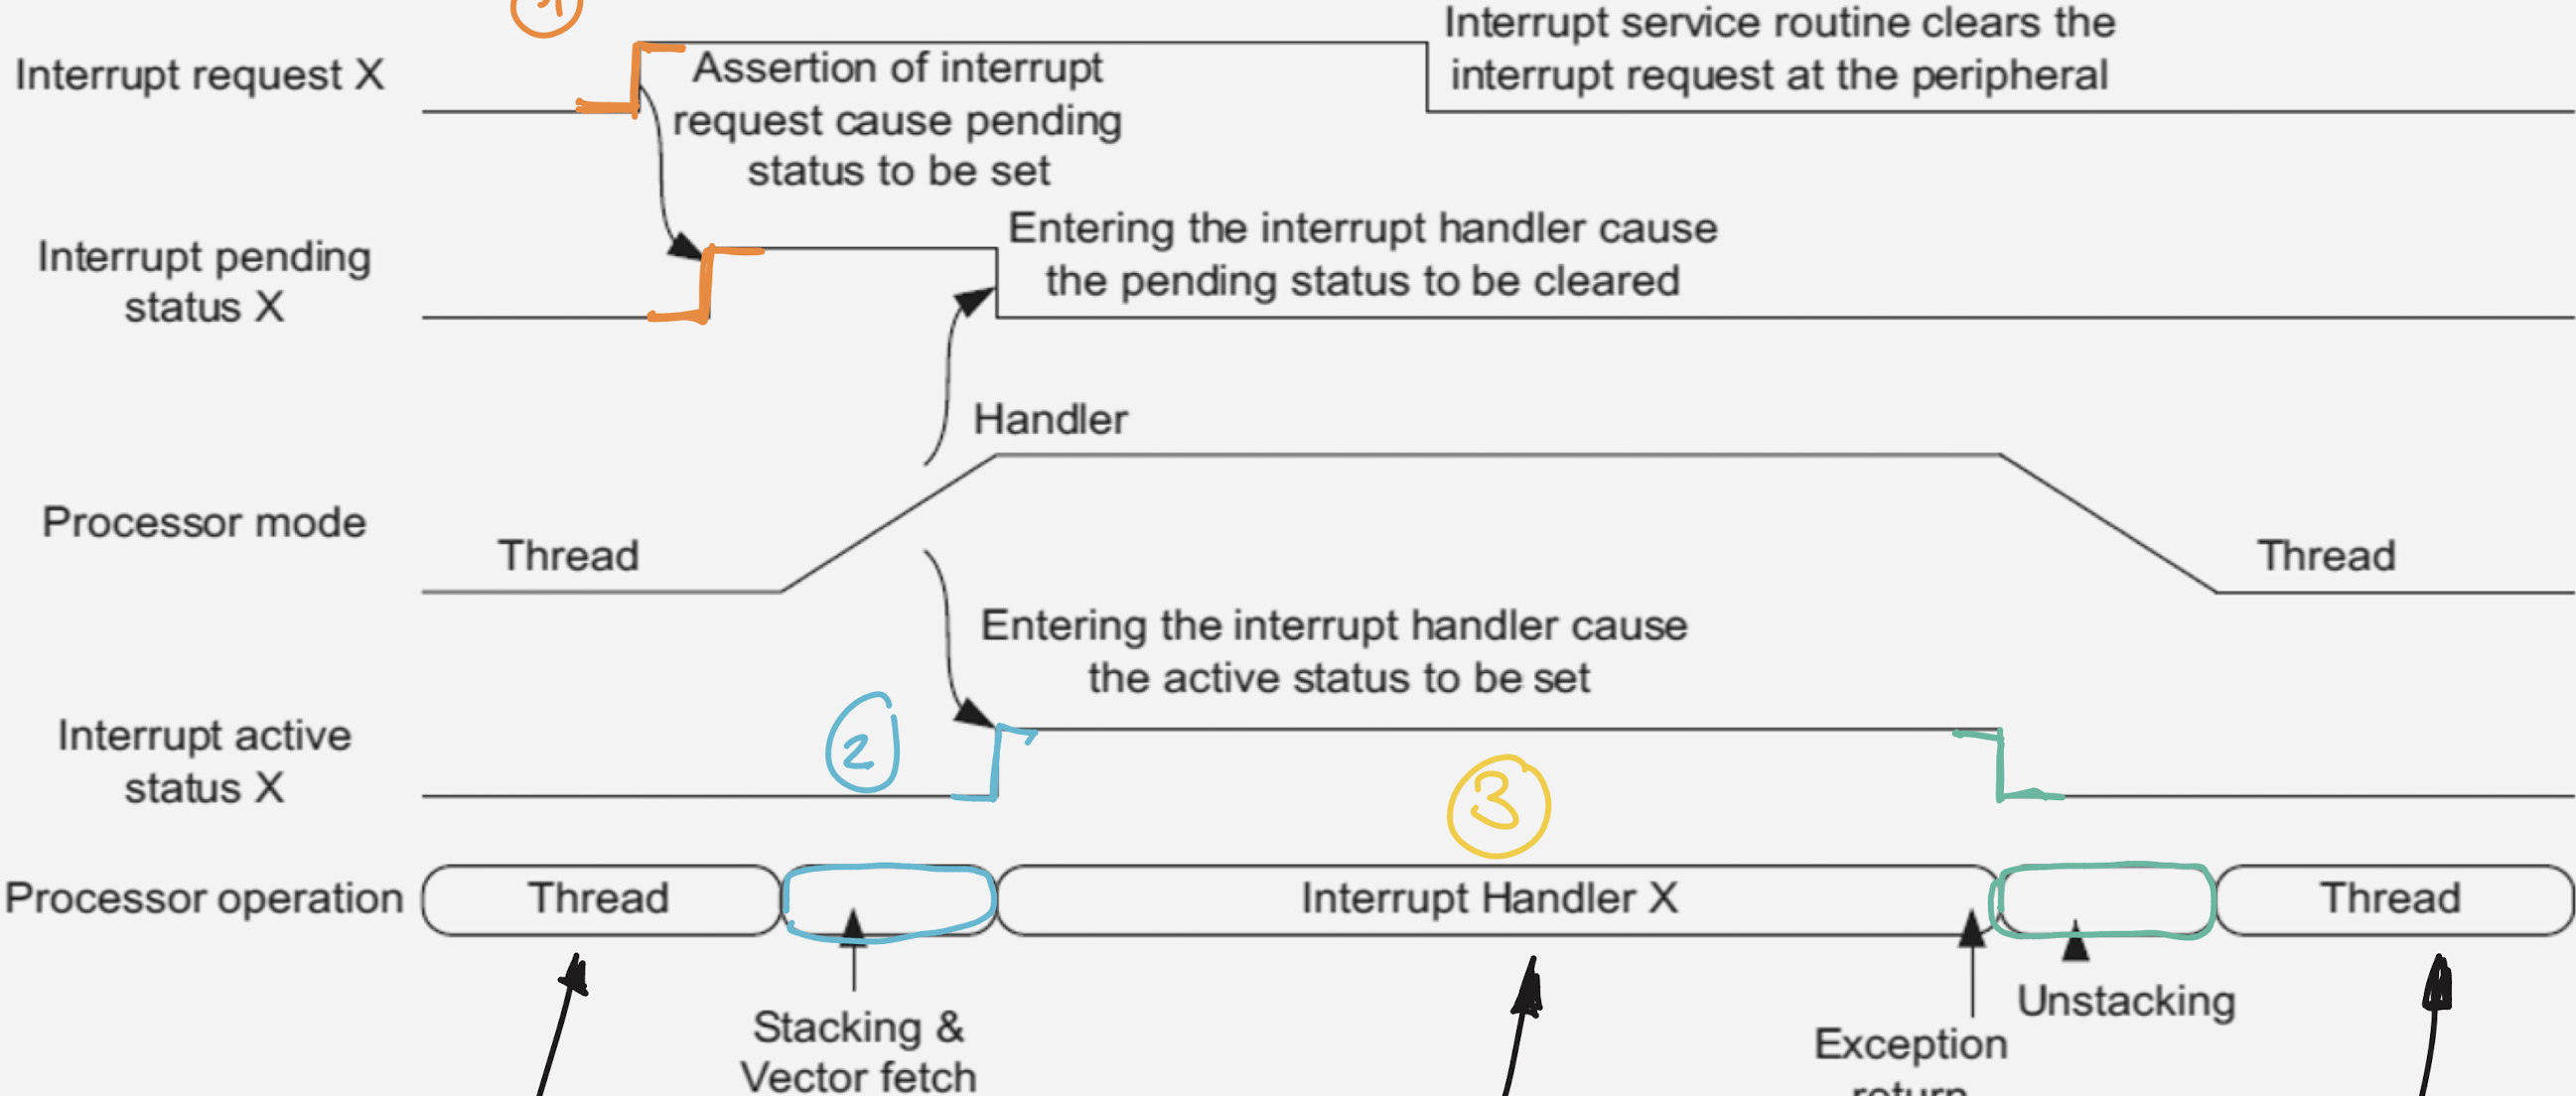
\includegraphics[width=\linewidth]{images/interrupt_vorgehen.png}
\end{minipage}